\chapter{Introduction}
\label{chap:introduction}


@introduction--- %where does this go?
Diminishing sea ice could lead to an increase in the aerosol number concentrations in the area where ice has retreated. The open sea surface it self would lead to an increase in release of sea salt and DMS to the lower atmosphere @cite. The lack of sea ice would also increase the likelyhood that the sea could be used for shipping, which would pollute the area @cite.
----


\textbf{Must rewrite: Aside from producing precipitation, clouds have a profound effect on our climate. If you consider the overall effect of all clouds on the surface temperature, they have a cooling effect because they block incoming solar radiation. However, the effect of an individual cloud depends on many factors such as its height, thickness, location, and whether it is day or night. .... tatt fra nettet, Colorado State, CMMAP}. Througout this thesis shortwave (SW) radiation means solar radiation and longwave (LW) radiation covers the terrestrial infrared radiation.

Here I will write my introduction. Needs a proper "målbeskrivelse"!
Something about how low clouds in the Arctic have a warming affect as opposed to the cooling effect they have on lower latitudes. This warming is due to the lack of SW radiation flux to reflect, and the emission of LW radiation flux to the ground therefore makes a greater difference.

(Something citing the IPCC report 2013 on the ice conditions in the Arctic, and something about Arctic clouds and radiation?)

Clouds are an important regulator of the Earth's radiation budget. They cover approximately 60\% of the Earth's surface~\citep{Lohmann2005}. It is well know that low clouds have a cooling effect at the surface due to their reflecting of incoming solar radiation. However, the effect is opposite in the Arctic, which I will elaborate on in Chapter~\ref{chap:theory} about clouds and radiation. Therefore it is important to investigate the changes in low clouds and their properties in the Arctic.

\section{Main goal}
With this thesis I strive to find if a decrease in Arctic sea ice lead to denser and more persistent clouds. It has been suggested that the decline in sea ice extent would allow for more pollution in the Arctic, as a consequence of more open water and ship traffic. The effect of increase in aerosol concentrations from shipping and open water, and the effect of enhanced evaporation from open water are studied separately and combined. With the main goal to find if this would lead to changes in clouds that could enhace downwelling longwave radiation and decrease upwelling shortwave radiation, both of which have warming effects.

\section{My contribution}
The findings in my thesis have been achived with some of the most recently developed code (by Greg Thompson) for cloud microphysics and aerosols and their effects on radiation, in modelling. The results build further on the work of many researchers @name-some-and-cite and contribute and may raise some questions for further research within the field.

\section{Area description}
The area of the study done in this thesis is in the Arctic, north of the United States of America and Canada. The study area covers the Beaufort Sea and a small part of Alaska and Canada, and can be seen in figure~\ref{fig:area}.

\begin{figure}
\centering
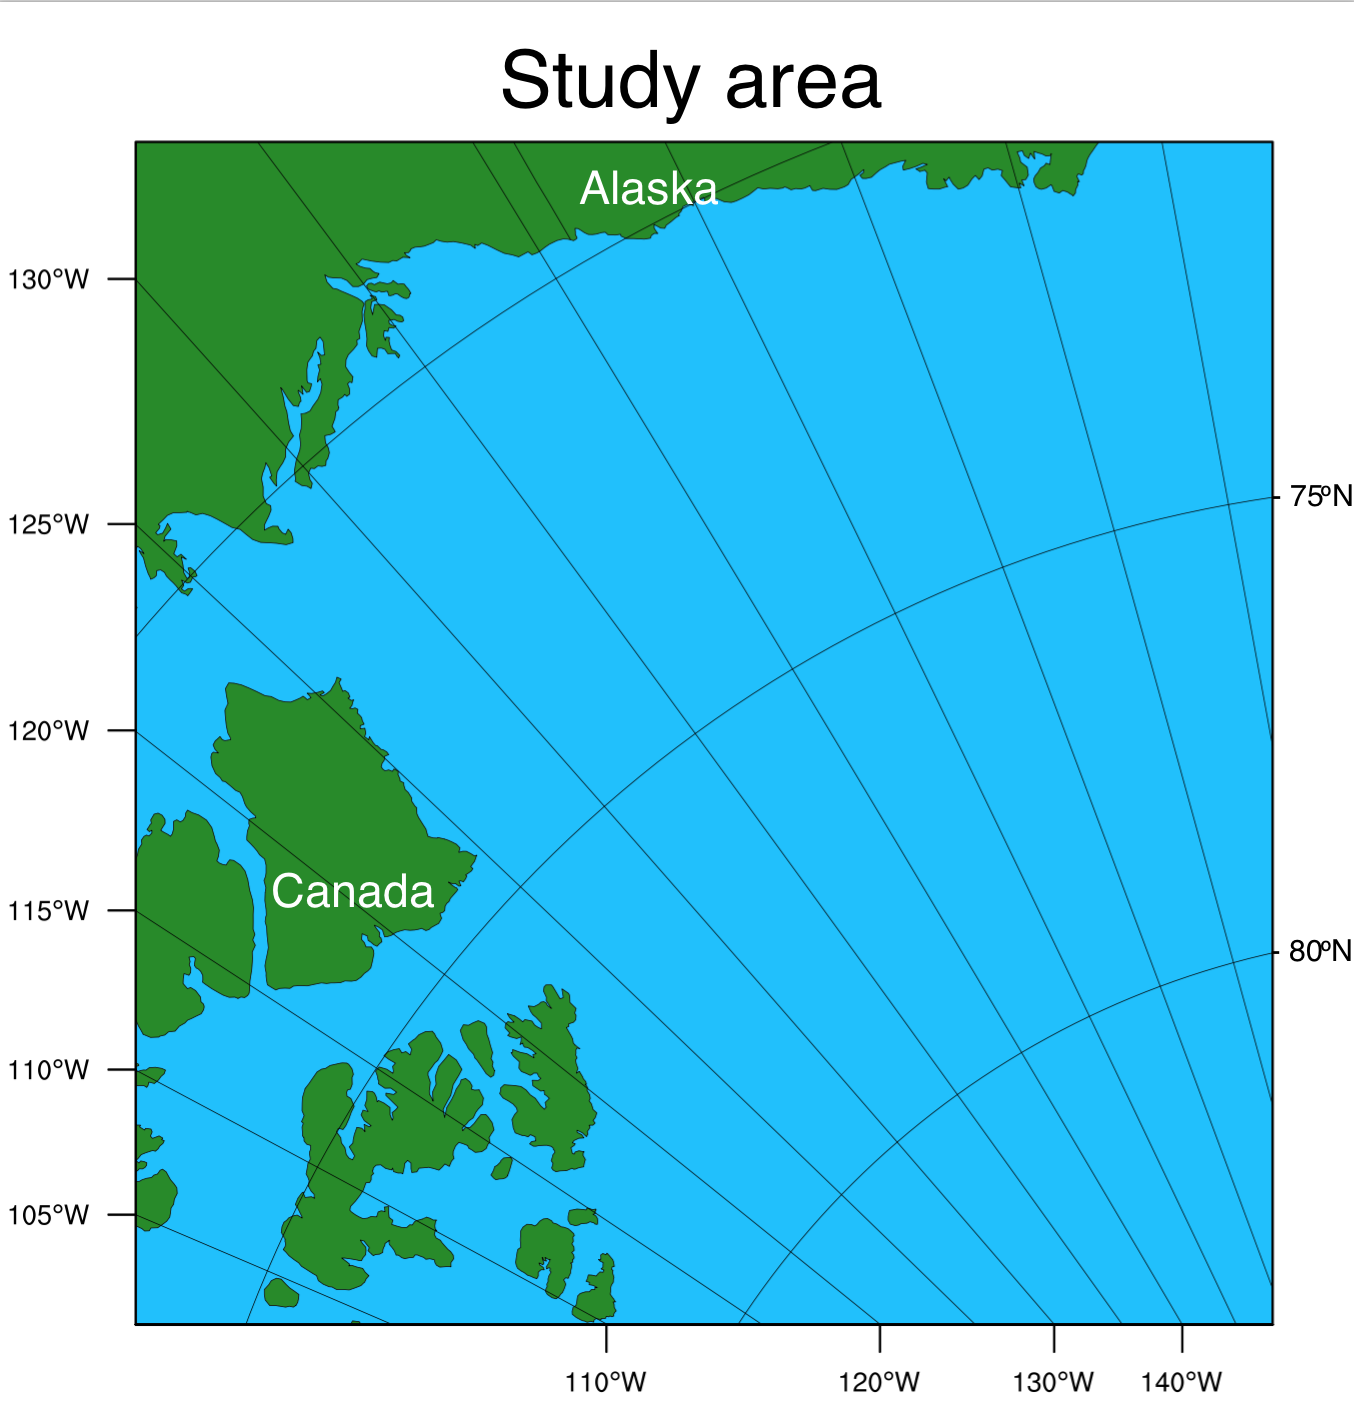
\includegraphics[width=0.7\textwidth]{introduction/studyarea.png}
\caption{An overview of the study area. The bottom right corner is the northernmost point and the y-axes show longitude and latitude to the left and right, respectivly.}
\label{fig:area}
\end{figure}
 

Here I should describe the area I have studied, and why it was chosen. Shown in figure~\ref{fig:area}.
The area was chosen because it had some ice in september, and because there have been research campaigns over the area with focus on clouds in the arctic (which is what I am studying). (show a map..?) Know the correct names of the seas and the land!!


\section{Structure of the thesis}
In the following chapter~\ref{chap:background} I will present the background for my thesis; what work I hope to compare my results to and relate my thesis to. Also I will touch upon why the subject of my thesis is important. In chapter~\ref{chap:theory} the most important theory and basic knowledge needed to understand some of the processes in clouds and their possible effect on the sea ice. Chapter~\ref{chap:modmet} is where I explain which model and tools and  I have used and how I have worked with them to get the results presented in chapter~\ref{chap:results}. The results are further discussed in chapter~\ref{chap:discussion}. A summary of main findings and conclusions are presented in the last chapter~\ref{chap:summaryconclusions}, before the list of references at the very end.


